\begin{tikzpicture}
	\pgfplotsset{/tikz/font={\small}}
	\begin{axis}[
		grid=both,
		width=1.0\textwidth,
		height=0.3\textheight,
		x tick label style={
		/pgf/number format/1000 sep=},
		ytick={0,-2,...,-26},
		y tick label style={
			/pgf/number format/.cd,
			fixed,
			fixed zerofill,
			precision=1,
		},
		y dir=reverse,
		ymax=0.5, ymin=-26,
		ylabel={Y BD-rate (\%)},
		% enlargelimits=0.15,
		enlarge y limits=false,
		enlarge x limits=0.04,
		legend style={at={(0.5,-0.45)},
		anchor=north,legend columns=-1},
		ybar interval,
		% bar width=1pt,
		xtick=data,
		xtick align=inside,
		% nodes near coords,
		% xlabel={Sequences},
		% xlabel near ticks,
		symbolic x coords={
			NebutaFestival,
			PeopleOnStreet,
			SteamLocTrain,
			Traffic,
			BasketballDrive,
			BQTerrace,
			Cactus,
			Kimono1,
			ParkScene,
			BasketballDrill,
			BQMall,
			PartyScene,
			RaceHorses\_480p,
			BasketballPass,
			BlowingBubbles,
			BQSquare,
			RaceHorses\_240p,
			FourPeople,
			Johnny,
			KristenAndSara,
			BasketDrillText,
			ChinaSpeed,
			SlideEditing,
			SlideShow,
			Overall,
		},
		x tick label style={rotate=-60,anchor=west},
		]

		\addlegendentry{Sep AI}
		\addplot coordinates {
		(NebutaFestival,   -1.06)
		(PeopleOnStreet,   -4.21)
		(SteamLocTrain,    -0.60)
		(Traffic,          -4.52)
		(BasketballDrive,  -3.22)
		(BQTerrace,        -4.70)
		(Cactus,           -5.22)
		(Kimono1,          -1.10)
		(ParkScene,        -4.61)
		(BasketballDrill,  -5.92)
		(BQMall,           -4.79)
		(PartyScene,       -4.88)
		(RaceHorses\_480p, -4.25)
		(BasketballPass,   -3.91)
		(BlowingBubbles,   -4.30)
		(BQSquare,         -4.58)
		(RaceHorses\_240p, -3.85)
		(FourPeople,       -4.56)
		(Johnny,           -3.34)
		(KristenAndSara,   -3.82)
		(BasketDrillText,  -6.24)
		(ChinaSpeed,       -4.25)
		(SlideEditing,     -4.80)
		(SlideShow,        -5.66)
		(Overall,          -4.10)
		};

		\addlegendentry{Sep RA}
		\addplot coordinates {
		(NebutaFestival,   -0.08)
		(PeopleOnStreet,   -1.49)
		(SteamLocTrain,     0.23)
		(Traffic,          -3.73)
		(BasketballDrive,  -0.72)
		(BQTerrace,        -2.65)
		(Cactus,           -3.08)
		(Kimono1,          -0.79)
		(ParkScene,        -3.22)
		(BasketballDrill,  -3.53)
		(BQMall,           -2.79)
		(PartyScene,       -3.21)
		(RaceHorses\_480p, -1.59)
		(BasketballPass,   -1.82)
		(BlowingBubbles,   -2.69)
		(BQSquare,         -2.74)
		(RaceHorses\_240p, -1.54)
		(FourPeople,       -5.18)
		(Johnny,           -4.16)
		(KristenAndSara,   -4.47)
		(BasketDrillText,  -3.71)
		(ChinaSpeed,       -2.71)
		(SlideEditing,     -5.05)
		(SlideShow,        -5.61)
		(Overall,          -2.76)
		};

























		\addlegendentry{N-sep AI}
		\addplot coordinates {
		(NebutaFestival,   -1.15)
		(PeopleOnStreet,   -5.65)
		(SteamLocTrain,    -0.68)
		(Traffic,          -6.06)
		(BasketballDrive,  -5.52)
		(BQTerrace,        -9.22)
		(Cactus,          -10.92)
		(Kimono1,          -1.80)
		(ParkScene,        -5.27)
		(BasketballDrill, -25.06)
		(BQMall,           -6.21)
		(PartyScene,       -6.19)
		(RaceHorses\_480p, -6.75)
		(BasketballPass,   -6.15)
		(BlowingBubbles,   -6.73)
		(BQSquare,         -6.12)
		(RaceHorses\_240p, -7.13)
		(FourPeople,       -6.33)
		(Johnny,           -5.21)
		(KristenAndSara,   -6.01)
		(BasketDrillText, -21.64)
		(ChinaSpeed,       -4.86)
		(SlideEditing,     -3.67)
		(SlideShow,        -6.03)
		(Overall,          -7.10)
		};

		\addlegendentry{N-sep RA}
		\addplot coordinates {
		(NebutaFestival,   -0.13)
		(PeopleOnStreet,   -2.27)
		(SteamLocTrain,     0.03)
		(Traffic,          -5.12)
		(BasketballDrive,  -2.36)
		(BQTerrace,        -4.93)
		(Cactus,           -7.68)
		(Kimono1,          -1.18)
		(ParkScene,        -3.69)
		(BasketballDrill, -14.80)
		(BQMall,           -3.64)
		(PartyScene,       -4.30)
		(RaceHorses\_480p, -3.24)
		(BasketballPass,   -3.14)
		(BlowingBubbles,   -3.95)
		(BQSquare,         -3.61)
		(RaceHorses\_240p, -3.20)
		(FourPeople,       -6.70)
		(Johnny,           -5.78)
		(KristenAndSara,   -6.17)
		(BasketDrillText, -13.15)
		(ChinaSpeed,       -3.03)
		(SlideEditing,     -4.06)
		(SlideShow,        -5.91)
		(Overall,          -4.67)
		};

	\end{axis}
\end{tikzpicture}
